% THIS TEMPLATE IS A WORK IN PROGRESS

\documentclass[polish, a4paper]{article}
\usepackage[a4paper,left=3cm,right=3cm,top=3cm,bottom=1.5cm]{geometry}
\usepackage[T1]{fontenc}
\usepackage[polish]{babel}
\usepackage[utf8]{inputenc}
\usepackage{hyperref}
\usepackage{fancyhdr}
\usepackage{float}
\usepackage{graphicx}
\usepackage{titling}
\usepackage{wasysym}
\usepackage{caption}
\usepackage{pgfplots}
\usepackage{pgfplotstable}
\usepackage{filecontents}
\usepackage{csvsimple}
\usepackage{textcomp}
\usepackage{gensymb}
\usepackage{etoolbox}
%\usepackage{siunitx}
\graphicspath{ {./} }
\pagestyle{fancy}

\setlength{\droptitle}{-1in}

%\lhead{\includegraphics[width=0.2\textwidth]{nyush-logo.pdf}}

  \lhead{Maciej Kaszkowiak}
  \chead{Warstwa łącza danych}
  \rhead{
  151856}


%%%% PROJECT TITLE
\title{Warstwa łącza danych \\
        \Large \emph{Sprawozdanie nr 3 z przedmiotu Sieci Komputerowe}}

%%%% NAMES OF ALL THE STUDENTS INVOLVED (first-name last-name)
\author{Maciej Kaszkowiak, 151856, zadania wykonane 1 kwietnia 2023}

\date{\vspace{-5ex}} %NO DATE


\begin{document}

\maketitle
%\thispagestyle{titlepage}

\tableofcontents

\newpage

\section{Zadanie 1}
\subsection{Przy pomocy programu wireshark przeanalizuj ruch w sieci
pod kątem występowania ramek Ethernet 802.3 i Ethernet v2.}

W sieci występują ramki zarówno typu Ethernet 802.3 jak i Ethernet v2.

\begin{figure}[H]
\centering
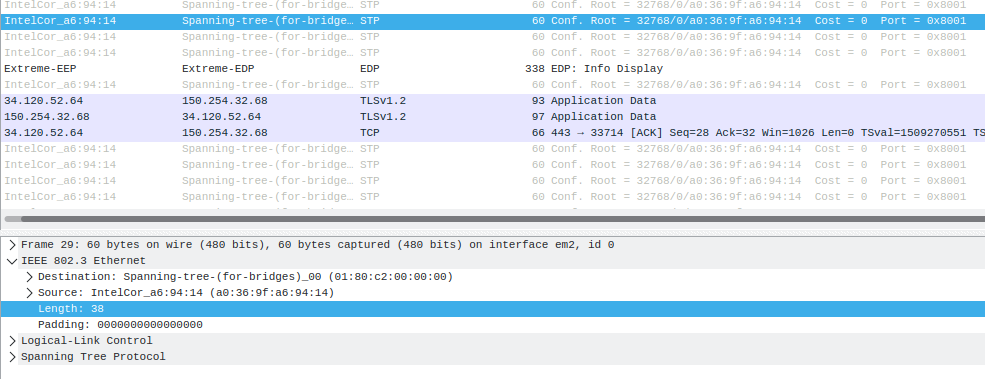
\includegraphics[width=\textwidth]{ieee8023.png}
\caption{Ramka STP typu Ethernet 802.3}
\end{figure}

\begin{figure}[H]
\centering
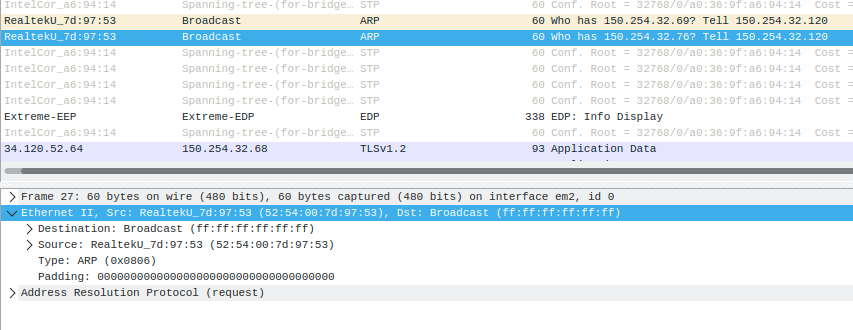
\includegraphics[width=\textwidth]{ethernetv2.png}
\caption{Ramka ARP typu Ethernet v2}
\end{figure}

\subsection{W przypadku jakich pakietów daje się zaobserwować ramki
Ethernet 802.3?}

Możemy zaobserwować ramki Ethernet 802.3 między innymi w przypadku pakietów z protokołami EDP, DTP, STP (Spanning Tree Protocol).

\section{Zadanie 2}
\subsection{Podłącz swój komputer (poprzez port p4p1) do koncentratora
(na zapleczu).}

Podłączyłem komputer poprzez port p4p1 do koncentratora na zapleczu.


\subsection{Skonfiguruj interfejs p4p1, tak by wszystkie komputery w
rzędzie działały w jednej sieci (unikalne sieci między rzędami).}

Wykonałem następującą komendę:
\begin{verbatim}
    lab-sec-3:/homex/student # ip addr add 192.168.1.3/24 dev p4p1
\end{verbatim}

\subsection{Przy pomocy programu wireshark przeanalizuj ruch na
interfejsie p4p1. Czy daje się zaobserwować pakiety z innych
sieci (w szczególności komunikaty protokołu telnet)?}

Tak, mogłem zaobserwować pakiety z innych sieci, w szczególności z protokołu telnet.

\begin{figure}[H]
\centering
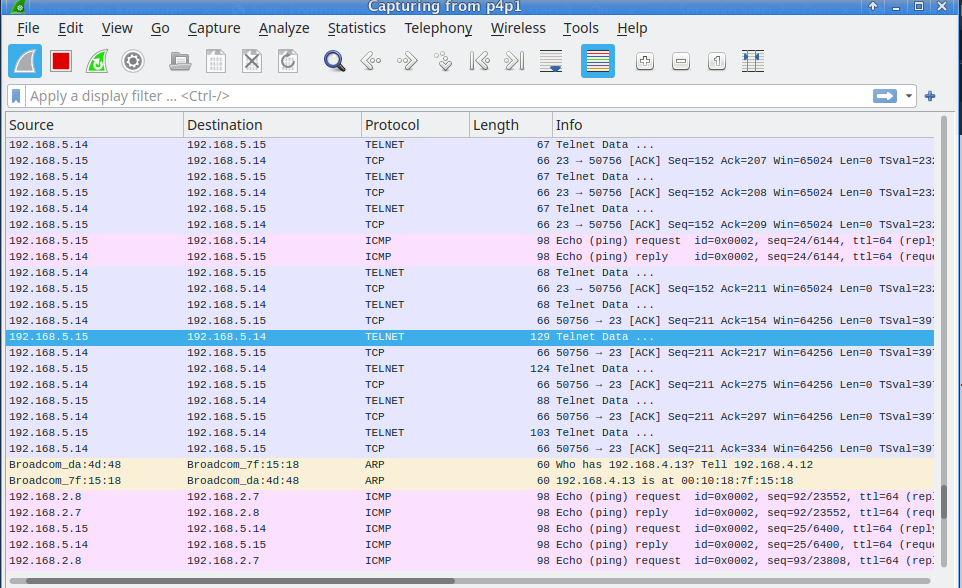
\includegraphics[width=\textwidth]{telnetidk.png}
\caption{Pakiety protokołu Telnet.}
\end{figure}

Musiałem również usunąć poprzednią konfigurację, a także wpiąć ponownie kabel do przełącznika (odpięcie wywołało stan DOWN).
\begin{verbatim}
    lab-sec-3:/homex/student # ip addr del 192.168.1.3/16 dev p4p1
\end{verbatim}

Po wpięciu kabla mogłem nawiązać ponownie transmisję:

\begin{verbatim}
lab-sec-3:/homex/student # ping 192.168.1.2
PING 192.168.1.2 (192.168.1.2) 56(84) bytes of data.
64 bytes from 192.168.1.2: icmp_seq=1 ttl=64 time=0.945 ms
64 bytes from 192.168.1.2: icmp_seq=2 ttl=64 time=0.709 ms
64 bytes from 192.168.1.2: icmp_seq=3 ttl=64 time=0.713 ms
\end{verbatim}


\section{Zadanie 3}
\subsection{W jednej chwili (wraz z koleżankami/kolegami) dokonaj
pomiaru prędkości transmisji z sąsiednim komputerem z tego
samego rzędu.}

Trzykrotnie uruchomiłem klient pomiaru transmisji w odstępach czasu. Pomiary prędkości różniły się w przedziale od 3 do 8 Mb/s.  

\begin{verbatim}
lab-sec-3:/homex/student # netperf -H 192.168.1.2
MIGRATED TCP STREAM TEST from 0.0.0.0 (0.0.0.0) port 0 AF_INET to 192.168.1.2 () port 0 AF_INET : demo
Recv   Send    Send                          
Socket Socket  Message  Elapsed              
Size   Size    Size     Time     Throughput  
bytes  bytes   bytes    secs.    10^6bits/sec  

131072  16384  16384    12.23       8.23   

lab-sec-3:/homex/student # netperf -H 192.168.1.2
MIGRATED TCP STREAM TEST from 0.0.0.0 (0.0.0.0) port 0 AF_INET to 192.168.1.2 () port 0 AF_INET : demo
Recv   Send    Send                          
Socket Socket  Message  Elapsed              
Size   Size    Size     Time     Throughput  
bytes  bytes   bytes    secs.    10^6bits/sec  

131072  16384  16384    12.98       6.35   
lab-sec-3:/homex/student # netperf -H 192.168.1.2
MIGRATED TCP STREAM TEST from 0.0.0.0 (0.0.0.0) port 0 AF_INET to 192.168.1.2 () port 0 AF_INET : demo
Recv   Send    Send                          
Socket Socket  Message  Elapsed              
Size   Size    Size     Time     Throughput  
bytes  bytes   bytes    secs.    10^6bits/sec  

131072  16384  16384    10.88       3.38   

\end{verbatim}

Wraz z rosnącą liczbą ludzi testujących jednocześnie przepustowość, można zauważyć że przepustowość w obrębie rzędu sukcesywnie malała.

\subsection{Wraz z innymi studentami zbadaj sumaryczną przepustowość
koncentratora.}

Wraz z innymi studentami zbadaliśmy sumaryczną przepustowość koncentratora. Do 8 kwietnia włącznie swoje odpowiedzi przesłały 4 osoby (6 Mb/s, 3.43 Mb/s, 5.56 Mb/s, 6.95 Mb/s). Suma przesłanych przepustowości wynosi 21.94 Mb/s - uważam natomiast, że nie stanowi to sumarycznej przepustowości koncentratora. Pomiary nie zostały wykonane w jednym momencie czasu, przez co chwilowa domena kolizyjna mogła być znacznie mniejsza. Na korzyść wymienionej tezy pragnę zauważyć, że pomiary wykonane przez mój rząd różniły się w zakresie od 3.38 do 8.23 Mb/s, w zależności od momentu uruchomienia testu.  

\section{Zadanie 4}
\subsection{Przepnij (na zapleczu) swój komputer do wspólnego
przełącznika i dokonaj ponownie pomiaru prędkości (jak w
poprzednim zadaniu).}

Możemy zaobserwować, że prędkość znacząco wzrosła do poziomu 941 Mb/s. (około 100-150 razy). Przede wszystkim: prędkość sieci jest stabilna oraz powtarzana pomiędzy testami.

\begin{verbatim}
lab-sec-3:/homex/student # netperf -H 192.168.1.2
MIGRATED TCP STREAM TEST from 0.0.0.0 (0.0.0.0) port 0 AF_INET to 192.168.1.2 () port 0 AF_INET : demo
Recv   Send    Send                          
Socket Socket  Message  Elapsed              
Size   Size    Size     Time     Throughput  
bytes  bytes   bytes    secs.    10^6bits/sec  

131072  16384  16384    10.03     941.36   
lab-sec-3:/homex/student # netperf -H 192.168.1.2
MIGRATED TCP STREAM TEST from 0.0.0.0 (0.0.0.0) port 0 AF_INET to 192.168.1.2 () port 0 AF_INET : demo
Recv   Send    Send                          
Socket Socket  Message  Elapsed              
Size   Size    Size     Time     Throughput  
bytes  bytes   bytes    secs.    10^6bits/sec  

131072  16384  16384    10.03     941.36   
lab-sec-3:/homex/student # netperf -H 192.168.1.2
MIGRATED TCP STREAM TEST from 0.0.0.0 (0.0.0.0) port 0 AF_INET to 192.168.1.2 () port 0 AF_INET : demo
Recv   Send    Send                          
Socket Socket  Message  Elapsed              
Size   Size    Size     Time     Throughput  
bytes  bytes   bytes    secs.    10^6bits/sec  

131072  16384  16384    10.03     941.36 
\end{verbatim}


\subsection{Skąd wynikają różnice w osiąganych prędkościach?}
Różnice w osiąganych prędkościach pomiędzy switchem a hubem spowodowane są nadmiernymi kolizjami w sieciach opartych o koncentrator.

\subsection{Czy w programie Wireshark można zobaczyć pakiety z
innych sieci? Jeśli tak to jakie?}
W programie Wireshark można zobaczyć pakiety w innych sieci, jednak są to pakiety tylko wybranych protokołów - zauważyłem m.in. protokoły SSDP.



\section{Zadanie 5}
\subsection{Wraz z koleżankami/kolegami przepnij połowę komputerów do
drugiego przełącznika, tak by komputery w parach były
podłączone do różnych przełączników.}
Mój komputer z numerem nieparzystym pozostał wpięty do pierwszego przełącznika.

\subsection{Przełączniki połącz ze sobą kablem (krosowanym).}
Dyżurny połączył przełączniki kablem krosowanym.

\subsection{Dokonaj ponownie pomiaru prędkości (jak w poprzednim
zadaniu).}

Pomiar prędkości na początku był niewykonalny:
\begin{verbatim}
    lab-sec-3:/homex/student # ping 192.168.1.2
PING 192.168.1.2 (192.168.1.2) 56(84) bytes of data.
64 bytes from 192.168.1.2: icmp_seq=79 ttl=64 time=81.4 ms
^C
--- 192.168.1.2 ping statistics ---
147 packets transmitted, 1 received, 99.3197% packet loss, time 149466ms
rtt min/avg/max/mdev = 81.398/81.398/81.398/0.000 ms
\end{verbatim}

Po zmianach prowadzącego w połączeniach sieć zaczęła działać.
Powód problemów z siecią: ktoś wpiął dwa końce jednego kabla do przełącznika.
\begin{verbatim}
    lab-sec-3:/homex/student # ping 192.168.1.2
PING 192.168.1.2 (192.168.1.2) 56(84) bytes of data.
64 bytes from 192.168.1.2: icmp_seq=20 ttl=64 time=7.76 ms
64 bytes from 192.168.1.2: icmp_seq=39 ttl=64 time=36.2 ms
64 bytes from 192.168.1.2: icmp_seq=39 ttl=64 time=36.5 ms (DUP!)
From 192.168.1.3 icmp_seq=74 Destination Host Unreachable
From 192.168.1.3 icmp_seq=75 Destination Host Unreachable
From 192.168.1.3 icmp_seq=76 Destination Host Unreachable
[...]
From 192.168.1.3 icmp_seq=95 Destination Host Unreachable
From 192.168.1.3 icmp_seq=96 Destination Host Unreachable
From 192.168.1.3 icmp_seq=97 Destination Host Unreachable
64 bytes from 192.168.1.2: icmp_seq=98 ttl=64 time=1025 ms
64 bytes from 192.168.1.2: icmp_seq=99 ttl=64 time=1.31 ms
64 bytes from 192.168.1.2: icmp_seq=100 ttl=64 time=0.698 ms
64 bytes from 192.168.1.2: icmp_seq=101 ttl=64 time=0.706 ms
[...]
64 bytes from 192.168.1.2: icmp_seq=131 ttl=64 time=0.713 ms
64 bytes from 192.168.1.2: icmp_seq=132 ttl=64 time=0.711 ms
64 bytes from 192.168.1.2: icmp_seq=133 ttl=64 time=0.340 ms
^C
--- 192.168.1.2 ping statistics ---
133 packets transmitted, 33 received, +1 duplicates, +24 errors, 75.188% packet loss, time 134969ms
rtt min/avg/max/mdev = 0.330/33.248/1025.326/172.902 ms, pipe 4
\end{verbatim}

Przeprowadziliśmy test prędkości:
\begin{verbatim}
    lab-sec-3:/homex/student # netperf -H 192.168.1.2
MIGRATED TCP STREAM TEST from 0.0.0.0 (0.0.0.0) port 0 AF_INET to 192.168.1.2 () port 0 AF_INET : demo
Recv   Send    Send                          
Socket Socket  Message  Elapsed              
Size   Size    Size     Time     Throughput  
bytes  bytes   bytes    secs.    10^6bits/sec  

131072  16384  16384    10.03     941.36   
\end{verbatim}


\subsection{Skąd wynikają różnice w osiąganych prędkościach?}
Prędkość mogłaby wzrosnąć ze względu na mniejszą domenę kolizyjną, jednak w teście pozostała ta sama.

\subsection{Czy można łatwo zwiększyć przepustowość?}
Tak, rozdzielając sieć na mniejsze podsieci.

\section{Zadanie 6}
\subsection{Dokonaj pomiaru prędkości transmisji do adresu 127.0.0.1.}
\begin{verbatim}
    lab-sec-3:/homex/student # netperf -H 127.0.0.1
MIGRATED TCP STREAM TEST from 0.0.0.0 (0.0.0.0) port 0 AF_INET to 127.0.0.1 () port 0 AF_INET : demo
Recv   Send    Send                          
Socket Socket  Message  Elapsed              
Size   Size    Size     Time     Throughput  
bytes  bytes   bytes    secs.    10^6bits/sec  

131072  16384  16384    10.00    90918.49 
\end{verbatim}

\subsection{Czy do tej transmisji angażowana jest karta sieciowa?}
Nie, pętlę zwrotną można wykorzystywać nawet bez karty sieciowej.

\section{Zadanie 7 }
\subsection{Podepnij swój komputer na porcie p4p1 do przełącznika, tak
by jeden przełącznik przypadał na jeden rząd w laboratorium.
Upewnij się, że działa połączenie z innymi komputerami w
rzędzie.}

Skonfigurowałem połączenie na porcie p4p1. Połączenie z innymi komputerami działa:

\begin{verbatim}
    lab-sec-3:/homex/student # ping 192.168.1.2
PING 192.168.1.2 (192.168.1.2) 56(84) bytes of data.
64 bytes from 192.168.1.2: icmp_seq=1 ttl=64 time=0.178 ms
64 bytes from 192.168.1.2: icmp_seq=2 ttl=64 time=0.206 ms
64 bytes from 192.168.1.2: icmp_seq=3 ttl=64 time=0.514 ms
64 bytes from 192.168.1.2: icmp_seq=4 ttl=64 time=0.254 ms
^C
--- 192.168.1.2 ping statistics ---
4 packets transmitted, 4 received, 0% packet loss, time 3059ms
rtt min/avg/max/mdev = 0.178/0.288/0.514/0.133 ms

\end{verbatim}


\subsection{Zepnij dwoma kablami przełącznik, do którego jest
podłączony Twój komputer z przełącznikiem odpowiadającym
sąsiedniemu rzędowi.}

Spięliśmy sąsiadujące przełączniki za pomocą kabli krosowych.

\subsection{Odpowiednio skonfiguruj interfejs p4p1 by móc skomunikować
się z siecią z sąsiedniego rzędu lub by dało się zaobserwować
jakikolwiek ruch w tamtej sieci.}

Skonfigurowałem interfejs p4p1 za pomocą następujących komend:

\begin{verbatim}
    lab-sec-3:/homex/student # ip addr del 192.168.1.3/24 dev p4p1
    lab-sec-3:/homex/student # ip addr add 192.168.1.3/16 dev p4p1
\end{verbatim}

Komunikacja nadal działa, zarówno w obrębie rzędu jak i całej sali:
\begin{verbatim}
    lab-sec-3:/homex/student # ping 192.168.1.2
PING 192.168.1.2 (192.168.1.2) 56(84) bytes of data.
64 bytes from 192.168.1.2: icmp_seq=1 ttl=64 time=0.367 ms
64 bytes from 192.168.1.2: icmp_seq=2 ttl=64 time=0.312 ms
64 bytes from 192.168.1.2: icmp_seq=3 ttl=64 time=0.457 ms
64 bytes from 192.168.1.2: icmp_seq=4 ttl=64 time=0.696 ms
64 bytes from 192.168.1.2: icmp_seq=5 ttl=64 time=0.699 ms
^C
--- 192.168.1.2 ping statistics ---
5 packets transmitted, 5 received, 0% packet loss, time 4082ms
rtt min/avg/max/mdev = 0.312/0.506/0.699/0.162 ms
lab-sec-3:/homex/student # ping 192.168.2.5
PING 192.168.2.5 (192.168.2.5) 56(84) bytes of data.
64 bytes from 192.168.2.5: icmp_seq=1 ttl=64 time=1.07 ms
64 bytes from 192.168.2.5: icmp_seq=2 ttl=64 time=0.693 ms
64 bytes from 192.168.2.5: icmp_seq=3 ttl=64 time=0.693 ms
64 bytes from 192.168.2.5: icmp_seq=4 ttl=64 time=0.247 ms
^C
--- 192.168.2.5 ping statistics ---
4 packets transmitted, 4 received, 0% packet loss, time 3041ms
rtt min/avg/max/mdev = 0.247/0.675/1.068/0.290 ms
\end{verbatim}

\subsection{Podglądaj ruch na interfejsie p4p1 przy pomocy programu
wireshark (najlepiej robić to tylko na jednym lub dwóch
wybranych komputerach w rzędzie).}

Możemy zaobserwować ruch w obrębie całej sali:

\begin{figure}[H]
\centering
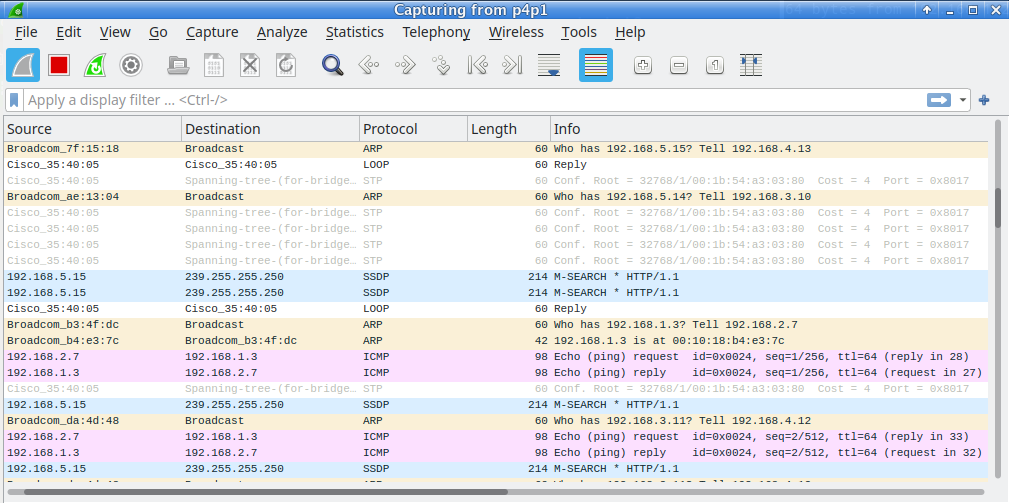
\includegraphics[width=\textwidth]{calasiec.png}
\caption{Ruch na interfejsie p4p1.}
\end{figure}

\subsection{Jeden z komputerów w rzędzie podepnij do wejścia
konsolowego przełącznika i uruchom (jako root) polecenie
picocom /dev/ttyS0. Zmień ustawienia/wykonaj polecenia
na przełączniku:}

\begin{itemize}
    \item terminate auto install: yes
    \item enter auto configuration: no
\item enable
\item configure terminal
\item no spanning-tree vlan 1
\end{itemize}

Zgodnie z poleceniem prowadzącego, zadanie zostało niewykonane przez brak czasu.

\subsection{Jeśli nie działoby się nic spektakularnego, wykonaj komendę
ping na adres z sieci zdefiniowanej dla rzędu, ale który jest
nieprzydzielony żadnemu komputerowi w laboratorium.}

Zgodnie z poleceniem prowadzącego, zadanie zostało niewykonane przez brak czasu.

\end{document}